
\section{DeepPicar}\label{sec:overview}

In this section, we provide an overview of our DeepPicar platform.
In developing DeepPicar, one of our primary goals is to faithfully
replicate NVIDIA's DAVE-2 system on a smaller scale using a low cost
multicore platform, the Raspberry Pi 3. Because Raspberry Pi 3's
computing performance is much lower than that of the DRIVE
PX~\cite{drivepx} platform used in DAVE-2, we are interested in if,
and how, we can process 
computationally expensive neural network operations in
real-time. Specifically, inferencing (forward pass processing)
operations must be completed within each control period
duration---e.g., a WCET of 33.3 ms for 30Hz control 
frequency---locally on the Pi 3 platform, although training of the 
network (back-propagation for weight updates) can be done offline and 
remotely using a desktop computer.

\begin{figure}[h]
  \centering
  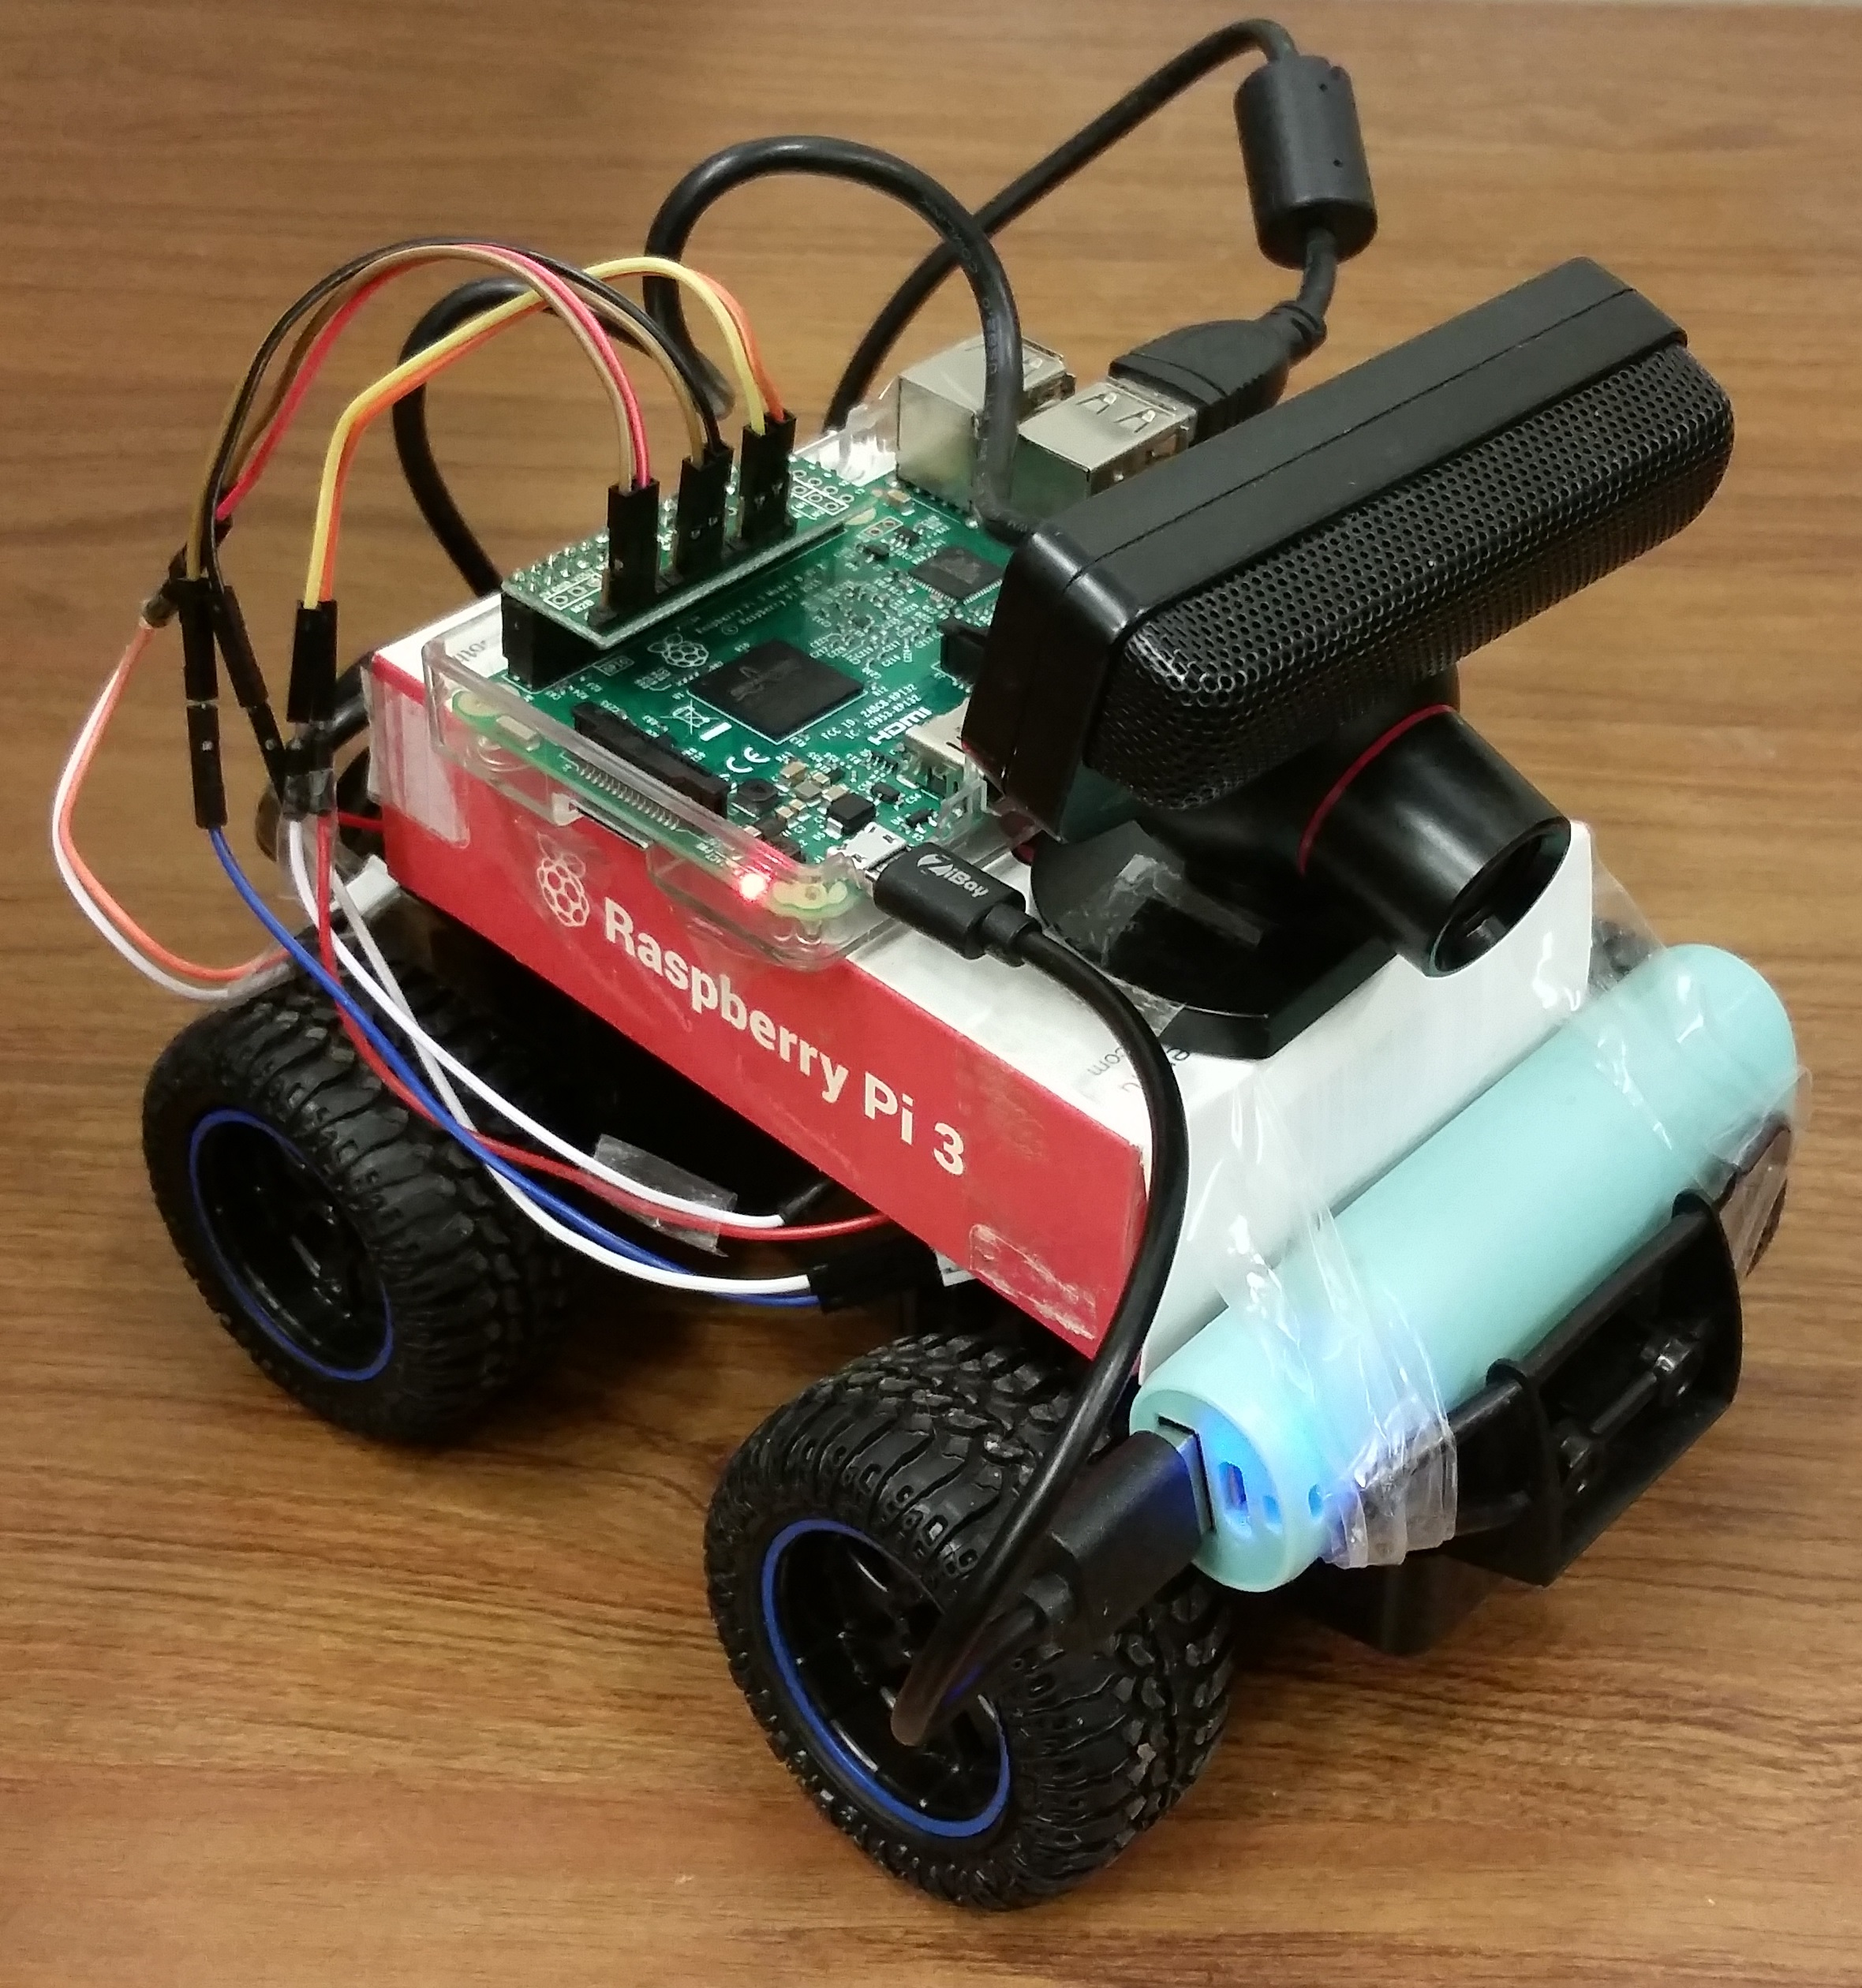
\includegraphics[width=.4\textwidth]{figs/DeepPicar_platform}
  \caption{DeepPicar platform.}
  \label{fig:overview}
\end{figure}

\begin{table}[h]
  \centering
  \begin{tabular}{|c|r|}
    \hline
    Item                    & Cost (\$) \\
    \hline
    Raspberry Pi 3 Model B  & 35 \\
    New Bright 1:24 scale RC car       & 10 \\
    Playstation Eye camera  &  7 \\
    Pololu DRV8835 motor hat&  8 \\
    External battery pack \& misc.   & 10 \\
    \hline
    Total                   & 70 \\
    \hline
  \end{tabular}
  \caption{DeepPicar's bill of materials (BOM)}
  \label{tbl:carbom}
\end{table}

Figure~\ref{fig:overview} shows the DeepPicar, which is comprised of a
set of inexpensive components: a Raspberry Pi 3 Single Board Computer
(SBC), a Pololu DRV8835 motor driver, a Playstation Eye webcam, a
battery, and a 1:24 scale RC car. Table~\ref{tbl:carbom} shows the
estimated cost of the system.

For the neural network architecture, we implement NVIDIA DAVE-2's
convolutional neural network (CNN) using an open-source CNN model in
~\cite{deeptesla}. Note, however, that the CNN model
in~\cite{deeptesla} is considerably larger than NVIDIA's CNN
model as it contains an additional fully-connected layer of
approximately 1.3M additional parameters. We remove the additional
layer to faithfully recreate NVIDIA's original CNN model.
%% The main difference is that we do not utilize a normalization layer, and 
%% instead initialize the weights using a Xavier initialization. 
As in DAVE-2, the CNN takes a raw color image (200x66 RGB pixels)
as input and produces a single steering angle value as output.
Figure~\ref{fig:architecture} shows the network architecture
used in this paper, which is comprised of 9 layers, 250K parameters,
and about 27 million connections as in NVIDIA DAVE-2's architecture.

\begin{figure}[h]
  \centering
  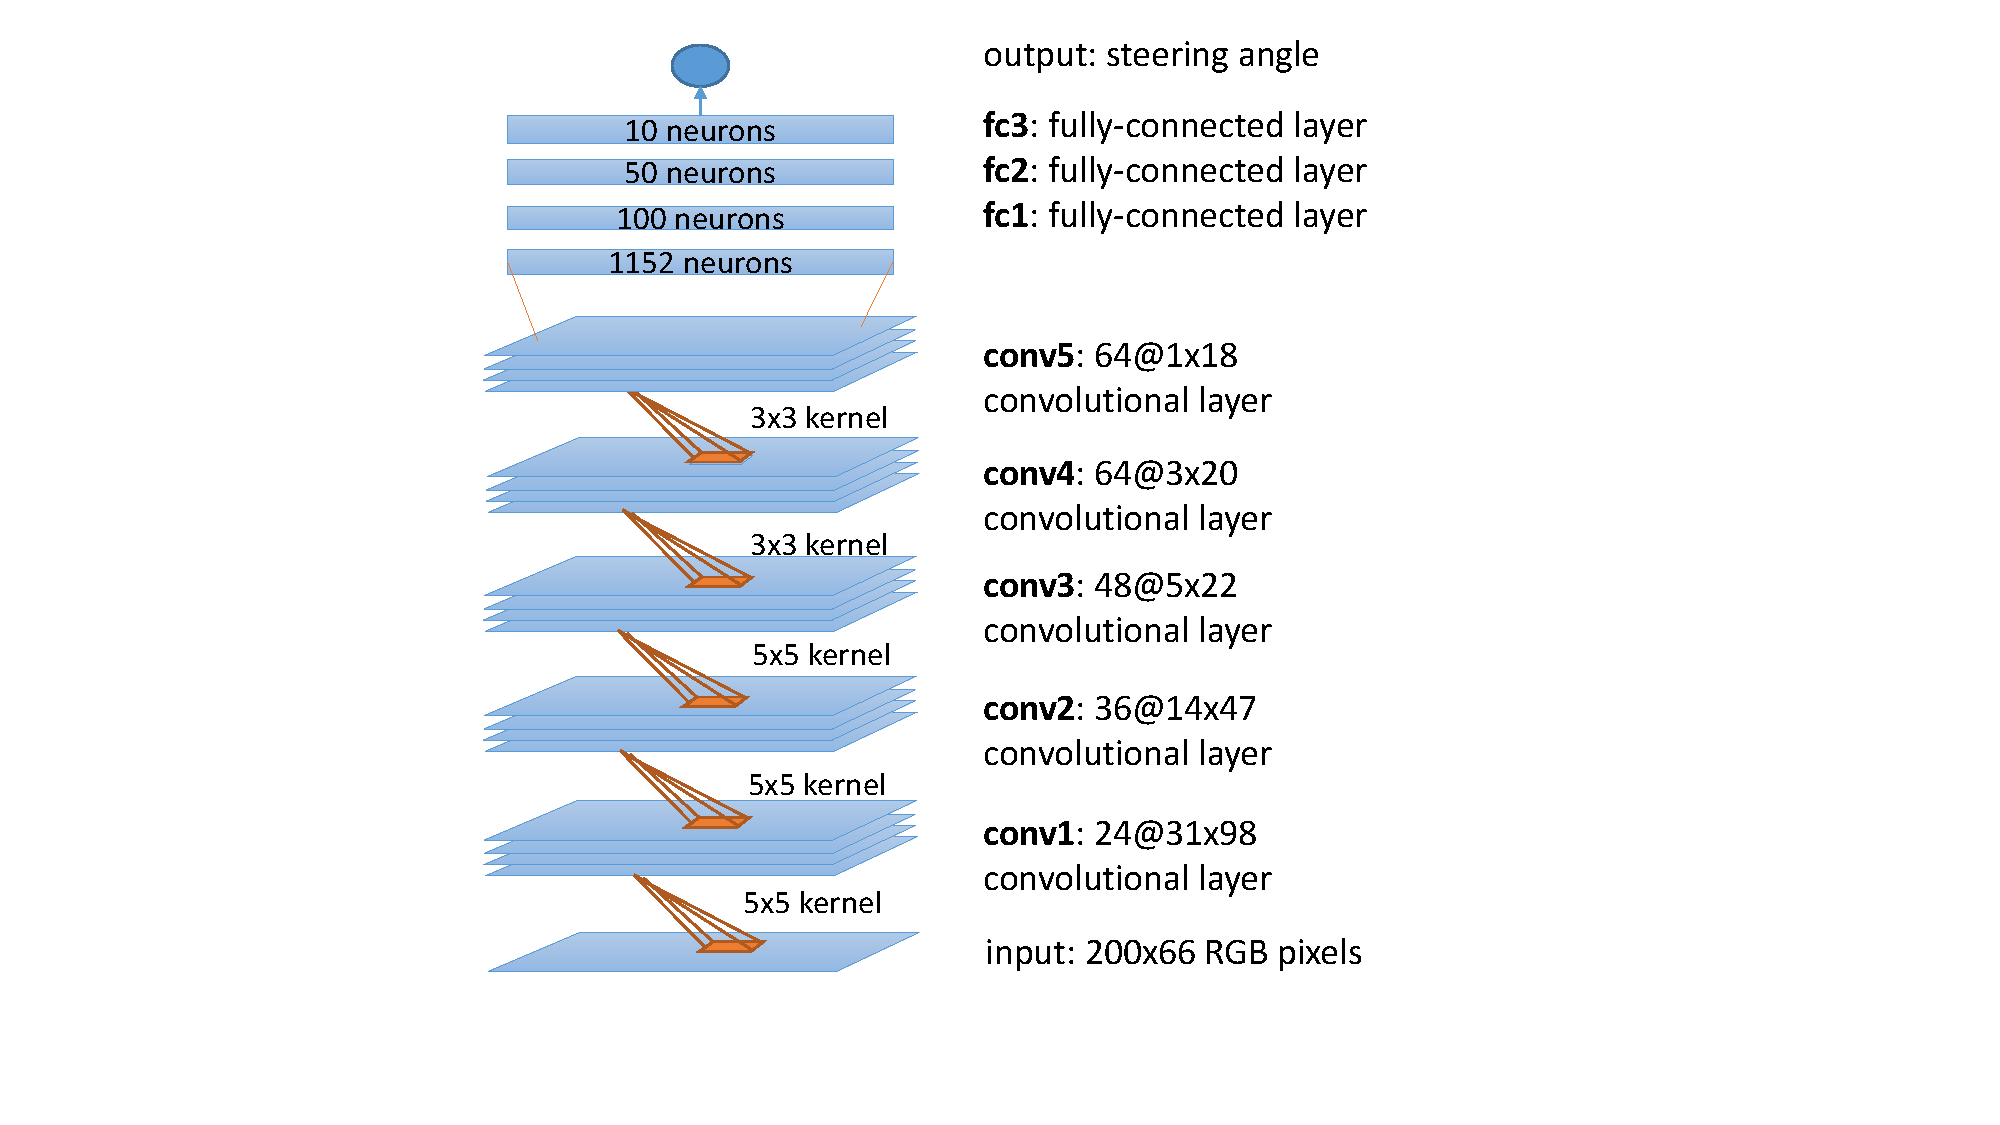
\includegraphics[width=0.4\textwidth]{figs/architecture}
  \caption{DeepPicar's neural network architecture: 9 layers (5
    convolutional, 4 fully-connected layers), 27 million connections,
    250K parameters. The CNN architecture is identical to the one 
	used in NVIDIA's real self-driving car~\cite{Bojarski2016}.}
  \label{fig:architecture}
\end{figure}


%% Note, however,
%% that we did not apply the normalization mentioned
%% in~\cite{Bojarski2016}, as it does not include trainable parameters
%% and its computational demand with respect to the overall CNN
%% processing is minimal.

\begin{figure}[h]
  \centering
  \begin{subfigure}{0.4\textwidth}
    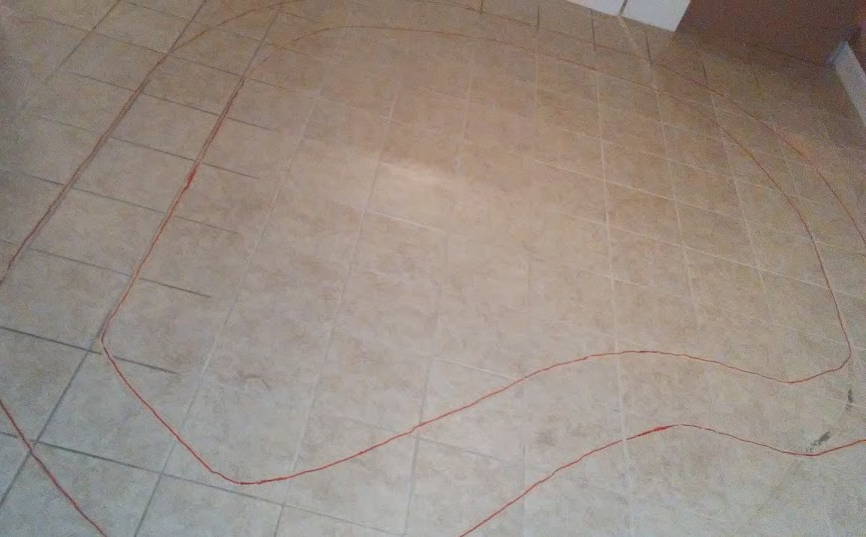
\includegraphics[width=\textwidth]{figs/track-2}
    \caption{Track 1.}
    \label{fig:track}
  \end{subfigure}
  \hfill
  \begin{subfigure}{0.4\textwidth}
    \includegraphics[width=\textwidth]{figs/track-3}
    \caption{Track 2.}
    \label{fig:track2}
  \end{subfigure}
  \caption{Custom tracks used for training/testing}
  \label{fig:tracks}
\end{figure}

% data collection and training.
To collect the training data, a human pilot manually drives the RC car
on tracks we created (Figure~\ref{fig:tracks}) to record
timestamped videos and contol commands. The stored data is then copied 
to a desktop computer, which is equipped with a NVIDIA Titan Xp GPU, 
where we train the network to accelerate training speed.

%% For comparison, training the network on the Raspbeery Pi 3 takes
%% approximately 4 hours, whereas it takes only about 4 minutes on the
%% desktop computer using the Titan Xp GPU.

\begin{figure}[h]
   \lstset{language=python,
           basicstyle=\ttfamily\small,
           keywordstyle=\color{blue}\ttfamily,
           stringstyle=\color{red}\ttfamily,
           commentstyle=\color{green}\ttfamily
          }  
  \lstinputlisting[language=python]{control.py}
  \caption{Control loop}
  \label{fig:controlloop}
\end{figure}

% inferencing on pi3
Once the network is trained on the desktop computer, the trained model
is copied back to the Raspberry Pi 3. The network is then used
by the car's main controlller, which feeds image frames from the web
camera as input to the network in real-time. At each control period,
the network produced steering angle output is converted into the PWM values
of the car's steering motor. Figure~\ref{fig:controlloop} shows simplified 
pseudo code of the controller's main loop. Among the five steps, the 3rd step, 
network inferencing, is the most computationally intensive and is expected to 
dominate the execution time.

Note that although the steering angle output of the CNN ($angle$) is
a continuous real value, the RC car we used only supports
three discrete angles---left (-30$^{\circ}$), center 
(0$^{\circ}$), and right (+30$^{\circ}$)---as control inputs.
We approximate the network generated real-valued angle to the closest
one of the three angles. Although this may introduce inaccuracy in
control, the observed control performance of the system is respectable,
likely due to the inherently stocastic nature of CNNs.

%% In the future, we plan to use a different (more expensive) RC car
%% platform that can precisely control the car's steering angle.

Another factors that can potentially affect the prediction accuracy of
the CNN, are camera and actuator (motor) control latencies. The camera
latency is from the time the camera sensor observes the scene to the
time the computer actually reads the digitized image data. This time
can be noticable depending on the camera used and the data processing
time of the computing platform. Higher camera latency could
negatively affect control performance, because the CNN would analyze
stale scenes. The actuator (motor) control latency from the time
the control output is sent to the steering motor to the time the motor
actually moved at a desired position, which also can takes
considerable time. In our platform, the combined latency is measured
to be around 50 ms, which is reasonble.
%% In other words, %% in the recorded video and control data, 
%% a control action of the CNN appears to be applied 50 ms later.
%% Considering that camera's framerate is 30Hz
%% (33.3 ms/frame), this is about two frames after the control action.
%% We experimentally measured the camera
%% latency and found it to be around 50-100 ms.
If this value is too high, control performance may suffer.
Our initial prototype suffered this problem as the observed latency
was as high as 300 ms, which negatively affected control performance.
For reference, the latency of human perception is known to be as fast
as 13 ms~\cite{ThomasBurger2015}. 
% https://www.pubnub.com/blog/2015-02-09-how-fast-is-realtime-human-perception-and-technology/

Our trained CNN models showed good prediction accuracy, successfully
navigating several different tracks we used for training.
For instance, the DeepPicar could remain on Track 1
(Figure~\ref{fig:track}) over 10 minutes at a moderate speed (50\%
throttle), at which point we stopped the experiment, and more than one
minute at a higher speed (75\% throttle)~\footnote{Self-driving videos: \url{https://photos.app.goo.gl/q40QFieD5iI9yXU42}
  %% \url{https://photos.app.goo.gl/ce93sU7jPk4ywO8u2}
}. Running at
higher speed is inherently more challenging because the CNN controller
has less time to recover from mistakes (bad predictions).  Also, we
find that the prediction accuracy is significantly affected by the
quality of training data as well as various environmental factors such
as lighting conditions. We plan to investigate more systematic ways
to improve the CNN's prediction accuracies.

We would like to stress, however, that
%% the issues related to the
%% CNN's accuracies have no impact on the \emph{computational 
%% aspects of the system}, and that 
our main focus of this study is not in improving the network accuracy
but in closely replicating the DAVE-2's network architecture and
studying its real-time characteristics, which will be presented in the
subsequent section.
